En esta sección se muestra el modelado 3D simplificado de los soportes y se realiza el analisis de esfuerzos y deformaciones sobre el soporte superior que es el que recibe la mayor carga.
\subsubsection{Suporte superior}
En la siguiente imagen se puede ver la forma general del soporte superior
\begin{figure}[H]
    \centering
        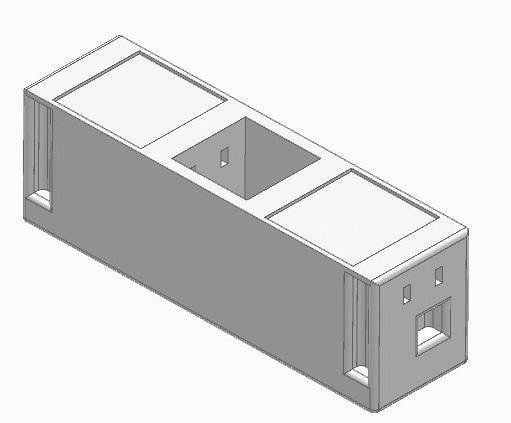
\includegraphics[width=0.65\textwidth]{img/SuperiorReal_simplificado_vista.jpg}
        \caption{\textit{Vista del soporte superior.}}
        \label{fig:SuperiorReal_simplificado_vista}
\end{figure}
A continuación se pueden observar las fuerzas aplicadas, siendo la carga máxima de aproximadamente 9kg. Las fuerzas se aplican sobre las caras que van atornilladas a los carros del perfil y sobre las caras que interactuan con las varillas.
\begin{figure}[H]
    \centering
        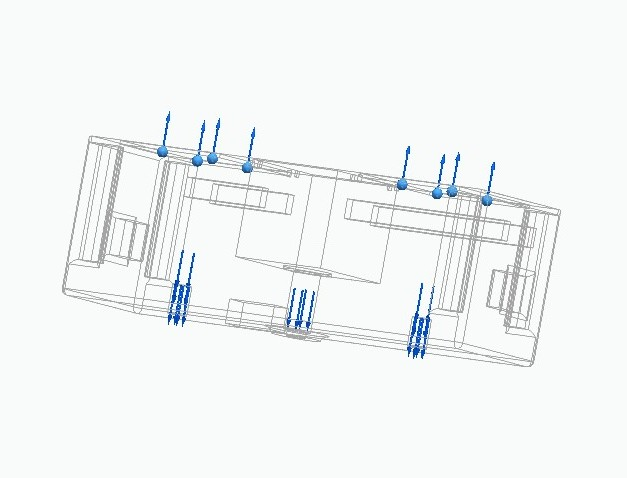
\includegraphics[width=0.65\textwidth]{img/SuperiorReal_simplificado_fuerzas_app.jpg}
        \caption{\textit{Cargas aplicadas sobre el soporte superior.}}
        \label{fig:SuperiorReal_simplificado_fuerzas_app}
\end{figure}

En la siguiente figura se puede observar que el diseño planteado es correcto y el material resiste a las fuerzas aplicadas ya que las deformaciones generadas son despreciables.
\begin{figure}[H]
    \centering
        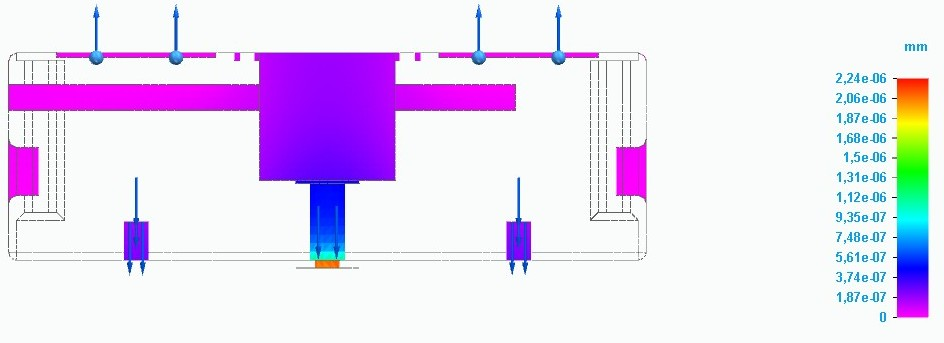
\includegraphics[width=0.65\textwidth]{img/SuperiorReal_simplificado_tensiones.jpg}
        \caption{\textit{Vista en corte del soporte donde se observan las deformaciones producidas por las fuerzas.}}
        \label{fig:SuperiorReal_simplificado_tensiones}
\end{figure}

\subsubsection{Suporte medio}
Este soporte se desplaza por el movimiento de la varilla, además es en donde se encuentra el brazo robótico y la cámara. Además posee un contrapeso del lado contrario al del brazo para mantener en equilibro el soprote.
\begin{figure}[H]
    \centering
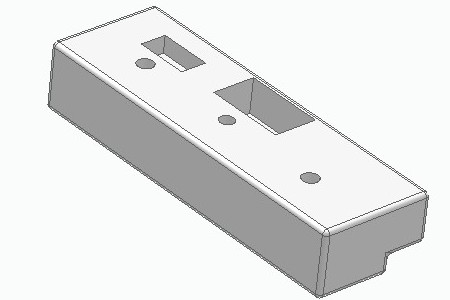
\includegraphics[width=0.65\textwidth]{img/MedioReal_simplificado_vista.jpg} \par
    \caption{\textit{Vista general del soporte medio.}}
    \label{fig:soporte_medio_Real}
\end{figure}

\subsubsection{Suporte inferior}
Este soporte cierra la estructura vertical, en él van los extremos de las varillas trefiladas y la varilla roscada y el final de carrera correspondiente. También cuenta con canales internos para el montaje de los cables. \\
\begin{figure}[H]
    \centering
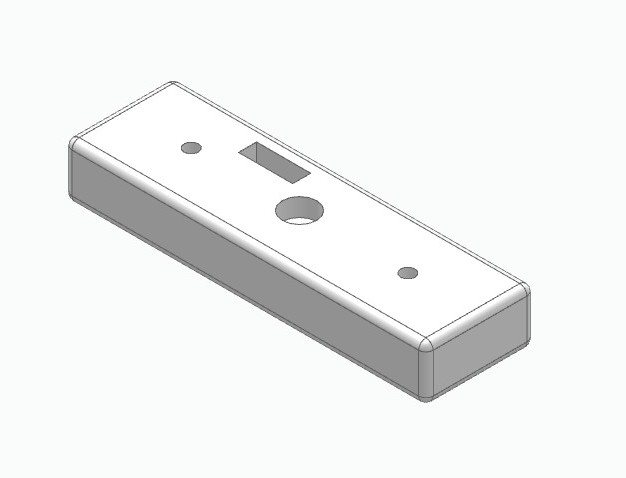
\includegraphics[width=0.65\textwidth]{img/InferiorReal_simplificado_vista.jpg} \par
    \caption{\textit{Soporte inferior.}}
    \label{fig:soporte_inferior_real}
\end{figure}

\subsubsection{Brazo robótico}
Para el diseño del brazo robótico se tienen 2 partes principales, el cuerpo del brazo y el efector final o gripper. Para este caso el material es PLA con fibra de carbono que es más rígido.
\begin{figure}[H]
    \centering
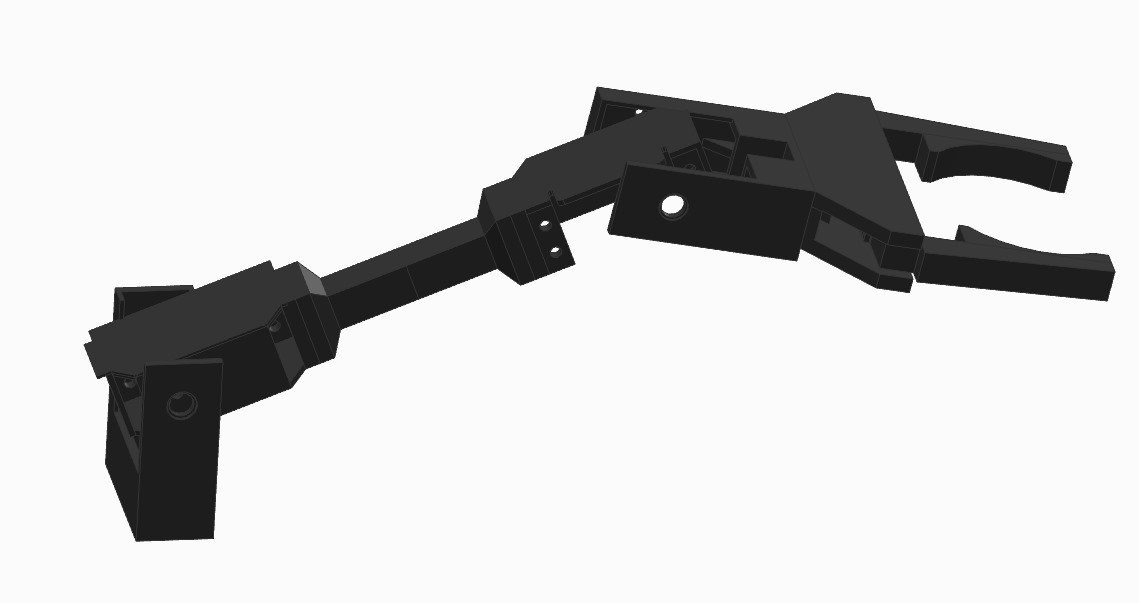
\includegraphics[width=0.65\textwidth]{img/brazo_completo.jpg} \par
    \caption{\textit{Brazo completo.}}
    \label{fig:brazo_Real}
\end{figure}
El diseño del gripper tiene en cuenta un sistema de transmisión piñon-cremallera para el agarre. 
\begin{figure}[H]
    \centering
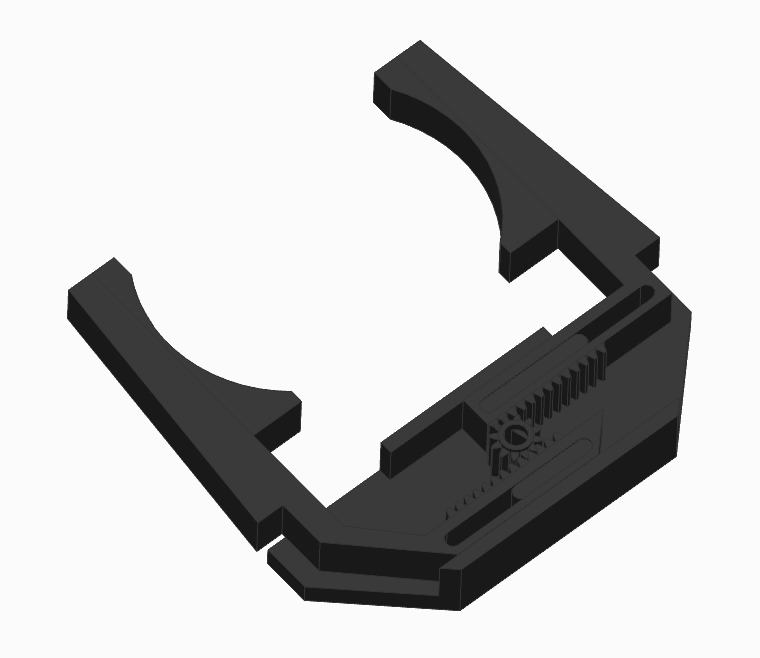
\includegraphics[width=0.65\textwidth]{img/gripper.jpg} \par
    \caption{\textit{Gripper.}}
    \label{fig:gripper_Real}
\end{figure}


